\documentclass[usenames, dvipsnames, t]{beamer}

%\usepackage{geometry}
%\geometry{legalpaper, textwidth=426pt}
%\usepackage[T1]{fontenc}
%\usepackage{fourier}
\usepackage{graphicx}
%\graphicspath{{Figures/}}
%
\usepackage[english]{babel}															% English language/hyphenation
%\usepackage[protrusion=true,expansion=true]{microtype}
\usepackage{amsmath,amsfonts,amsthm} % Math packages
\usefonttheme[onlymath]{serif}
\usepackage{graphicx, adjustbox}
\graphicspath{{figures/}}
%\usepackage{url}
\newcommand{\red}[1]{\textcolor{red}{#1}}
\newcommand{\blue}[1]{\textcolor{blue}{#1}}
%
%% Self included packages
%%\usepackage[labelfont=sf,			hypcap=false,			format=hang,			width=\columnwidth]{caption}
%\usepackage{amsmath}
%\usepackage{wrapfig}
\usepackage[ruled, vlined]{algorithm2e}
\usepackage{pgfplots}
%\pgfplotsset{soldot/.style={color=blue,only marks,mark=*}} \pgfplotsset{holdot/.style={color=blue,fill=white,only marks,mark=*}}
\pgfplotsset{compat=1.12}
\usepackage{xcolor}
\usepackage{tikz}
\usetikzlibrary{graphs, graphs.standard, shapes.misc, positioning, fit, shadows, calc, snakes, shapes, patterns, arrows.meta, matrix, shapes.geometric}
% \usepackage[noend]{algpseudocode}
\usepackage{hyperref}
\hypersetup{
    colorlinks,
    citecolor=black,
    filecolor=black,
    linkcolor=black,
    urlcolor=black
}
%\usepackage{ifthen}
\usepackage{bm}
%\usepackage{enumerate}
%%%%%%%%%%%%%%%%%%%%%%%%%%%%%%%%%%%%%%%%%%%%%%%%%%%%%%%%%%%%%%%%%%%%%%%%%%%
\usetheme{CambridgeUS}
\usecolortheme{beaver}
\usepackage[english]{babel}

\setbeamertemplate{section in toc}{\inserttocsection}
\setbeamertemplate{subsection in toc}{\hspace{1.2em}~\inserttocsubsection\par}

\setbeamerfont{section in toc}{size=\small}
\setbeamerfont{subsection in toc}{size=\footnotesize}

\setbeamertemplate{itemize item}{\color{red}$\circ$}
\setbeamertemplate{itemize subitem}{\color{red}$\circ$}

\setbeamertemplate{enumerate item}[default]
\setbeamercolor*{enumerate item}{fg=red}
\setbeamercolor*{enumerate subitem}{fg=red}
\setbeamercolor*{enumerate subsubitem}{fg=red}

\setbeamertemplate{footline}
{
  \leavevmode%
  \hbox{%
  \begin{beamercolorbox}[wd=.2\paperwidth,ht=2.25ex,dp=1ex,center]{author in head/foot}%
  	\usebeamerfont{author in head/foot}\insertshortauthor
  \end{beamercolorbox}%

  \begin{beamercolorbox}[wd=.5\paperwidth,ht=2.25ex,dp=1ex,center]{title in head/foot}%
    	\usebeamerfont{title in head/foot}\insertshorttitle\hspace*{3em}
  \end{beamercolorbox}%

  \begin{beamercolorbox}[wd=.3\paperwidth,ht=2.25ex,dp=1ex,right]{date in head/foot}%
    	\usebeamerfont{date in head/foot}\insertshortdate{}\hspace*{2em}
	\insertframenumber{} / \inserttotalframenumber\hspace*{2ex}
  \end{beamercolorbox}}%
  \vskip0pt%
}

\title{Interpolation of Molecular Dynamics with Bi-Directional Neural Networks}
\subtitle{}
\author{Ludwig Winkler \& Huziel Sauceda}
\date{\today}


%%%%%%%%%%%%%%%%%%%%%%%%%%%%%%%%%%%%%%%%%%%%%%%%%%%%%%%%%%%%%%%%%%%%%%%%%%%%
\begin{document}

\def\mathn#1{\mathnormal{#1}}
\def\thet{\bm{\theta}}
\def\V{\mathn{V}}
\def\Q{\mathn{Q}}
\def\R{\mathn{R}}
\def\r{\mathn{r}}
\def\G{\mathn{G}}
\def\n{\mathn{n}}
\def\A{\mathn{A}}
\def\T{\mathn{T}}
\def\W{\mathn{W}}
% \def\E{\mathbb{E}}

\def\w{\mathn{w}}
\def\p{\mathn{p}}
\def\q{\mathn{q}}
\def\a{\mathn{a}}
\def\r{\mathn{r}}
\def\s{\mathn{s}}
\def\t{\mathn{t}}
\def\dist{1}

\newcommand{\E}{\mathbb{E}}

\tikzset{ shorten <>/.style={ shorten >=#1, shorten <=#1 } }


\begin{frame}
	\titlepage
\end{frame}

% \begin{frame}
% \frametitle{Outline}
% \tableofcontents
% \end{frame}

\begin{frame}
	\frametitle{Bi-Directional Interpolation of Differential Equation}
	\begin{itemize}
		\item Can we predict MD trajectories directly with a neural network (NN)?
		\item[] 
		\item Use NN to predict solver for MD equations
		\item NN are trained on predicting change in position and momentum
		\item[]  
		\item But we still want the accuracy of real MD simulations?
		\item[]   
		\item Use coarse grained MD simulation to predict initial and final conditions of differential equation governing MD trajectories
		\item Reconstruct high dimensional components to interpolate smartly with NN between coarse grained solution
	\end{itemize}
\end{frame}

\begin{frame}
	\frametitle{Bi-Directional Interpolation of Differential Equation}
	\begin{itemize}
		\item Given true dynamics $f$ learn approximate dynamics $f_\theta$ with NN
		\item Train $f_\theta$ to predict the true solutions $x(t)$
		\item[] 
		\item Integrate approximate dynamics $f_\theta$ to obtain approximate solution $\hat{x}(t)$
		\item[]   
		\item Use coarse grained MD simulation to predict initial and final conditions of differential equation governing MD trajectories
		\item Reconstruct high dimensional components to interpolate smartly with NN between coarse grained solution
	\end{itemize}
\end{frame}

\begin{frame}
	\frametitle{Bi-Directional Interpolation of Differential Equation}
	\begin{itemize}
		\item Predict forward solution \red{$\overrightarrow{\hat{x}(t)}$} and backward solution \blue{$\overleftarrow{\hat{x}(t)}$} with the \textbf{same} dynamics $f_\theta$
		\item Use adiabatic connection to interpolate \red{$\overrightarrow{\hat{x}(t)}$} and \blue{$\overleftarrow{\hat{x}(t)}$} to $\hat{x}(t)$
		\begin{align}
			\hat{x}(t) = (1-\lambda(t)) \ \red{\overrightarrow{\hat{x}(t)}} + \lambda(t) \ \blue{\overleftarrow{\hat{x}(t)}}
		\end{align}
	\end{itemize}
	% \resizebox*{0.5\textwidth}{1.2\textheight}{
	\begin{figure}
		% \centering
		\begin{adjustbox}{max width = 1.\textwidth, height = 0.5\textheight}
			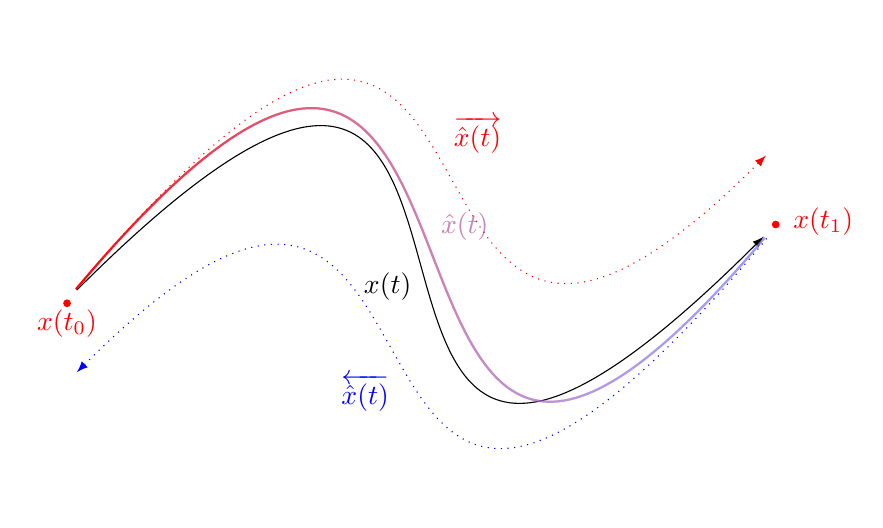
\begin{tikzpicture}
			\tikzset{arrow/.style={-latex, shorten >= 5pt, shorten <= 5pt}}
			\tikzset{diff/.style={-latex, shorten >= 5pt, shorten <= 5pt}}
			\tikzset{node/.style={draw, circle, fill, red, scale=0.25}}

			\clip (-0.5,3) rectangle (10,-3);
			
			\node (z0) [node, label={[below, red]{$x(t_0)$}}] at (0,-0.5) {}; 
			\node (zT) [node, label={[right=0.1cm, red]{$x(t_1)$}}] at (9, 0.5) {};
			\draw[arrow, black] (z0.north) .. controls +(45:10cm) and +(225:10cm) .. node[below left]{$x(t)$} (zT);
			\draw[shorten >= 5pt, shorten <= 5pt, , red, thick, path fading=east] (z0.north) .. controls +(50:10cm) and +(230:9.5cm) .. node[above right]{$\hat{x}(t)$} (zT);
			\draw[shorten >= 5pt, shorten <= 5pt, blue!50, thick, path fading=west, opacity=0.8] (z0.north) .. controls +(50:10cm) and +(230:9.5cm) .. node[above right]{$\hat{x}(t)$} (zT);
			
			\draw[arrow, dotted, red] (z0.north) .. controls +(50:10cm) and +(225:8cm) .. node[above right]{$\overrightarrow{\hat{x}(t)}$} ($(zT)+(0cm,1cm)$);
			
			% \draw[draw=none] (z0.north) .. controls +(50:10cm) and +(225:8cm) .. node[above right]{$\overrightarrow{\hat{x}(t)}$} ($(zT)+(0cm,1cm)$)
				% \foreach \t in {25, 50, 75, 90, 100}
					% { node[red] (forward\t) [pos=\t/100,node,draw=red] {} };
			
			% \draw[arrow, dotted, red] (z0) to (forward);
			% \foreach \s/\e in {25/50, 50/75, 75/90, 90/100}
			% 	{
			% 	\draw[arrow, dotted, red] (forward\s) to (forward\e);
			% 	}
			
			\draw[arrow, dotted, blue] (zT.south) .. controls +(230:10cm) and +(45:8cm) .. node[below left]{$\overleftarrow{\hat{x}(t)}$}($(z0)+(0cm,-1cm)$);
		
			\end{tikzpicture}
		% }
		\end{adjustbox}
	\end{figure}
\end{frame}

\begin{frame}
	\frametitle{Bi-Directional Interpolation of Differential Equation}
	\begin{itemize}
		 \item Unidirectional LSTM architecture for Benzene MD trajectory interpolating over 20 time steps
	\end{itemize}
	\begin{figure}
		 \centering
		 \includegraphics[width=0.8\textwidth]{ExampleTrajectory.png}
	\end{figure}
\end{frame}

\begin{frame}
	\frametitle{Bi-Directional Interpolation of Differential Equation}
	\begin{itemize}
		 \item Bidirectional LSTM architecture for Benzene MD trajectory interpolating over 20 time steps
		 \item Final condition and additional bidirectional training smooth trajectories significantely
	\end{itemize}
	\begin{figure}
		 \centering
		 \includegraphics[width=0.8\textwidth]{ExampleTrajectoryBi.png}
	\end{figure}
\end{frame}

\end{document}
